\begin{exercice*}
    \phantom{rrr}

    \begin{minipage}{0.7\linewidth}        
        Le figure ci-contre représente deux cônes de sommet $S$.
        \begin{itemize}
            \item $[SB]$ et $[SH]$ sont les
            
            hauteurs des cônes.
            \item $H$, $B$ et $S$ sont alignés.
            \item $A$, $S$ et $J$ sont alignés.
            \item $HJ=\Lg{7.3}$.
            \item $HB=\Lg{7.8}$.
            \item $BS=\Lg{2.6}$.
        \end{itemize}

        \vspace*{10mm}
        Calculer la mesure du rayon $[AB]$.
    \end{minipage}
    \begin{minipage}{0.3\linewidth}    
    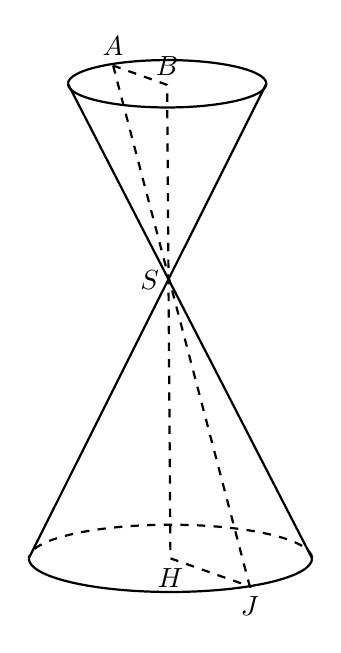
\begin{tikzpicture}[scale=0.7]
        % \draw[help lines, color=black!30, dashed] (0,0) grid (8,12);        
        \coordinate[label=above:$A$] (A) at (3.46,10.94);
        \coordinate[label=above:$B$] (B) at (4.44,10.59);
        \coordinate[label=below:$H$] (H) at (4.5,2);
        \coordinate[label=below:$J$] (J) at (5.94,1.49);
        \coordinate[label=left:$S$] (S) at (4.47,7.05);
        \coordinate (H1) at (7.07,2);
        \coordinate (H2) at (1.93,2);
        \coordinate (L1) at (6.24,10.61);
        \coordinate (L2) at (2.64,10.61);
        \draw[thick, dashed] (H1) arc(0:180:25.7mm and 6.10mm);
        \draw[thick] (H2) arc(180:360:25.7mm and 6.10mm);
        \draw[thick] (L1) arc(0:180:18mm and 4.3mm);
        \draw[thick] (L2) arc(180:360:18mm and 4.3mm);
        \draw[thick,dashed] (A)--(J)--(H)--(B)--(A);
        \draw[thick] (L1)--(H2);
        \draw[thick] (L2)--(H1);
    \end{tikzpicture}
    \end{minipage}
\end{exercice*}
\begin{corrige}
    %\setcounter{partie}{0} % Pour s'assurer que le compteur de \partie est à zéro dans les corrigés
    \phantom{rrr}

    \begin{itemize}

    \item Comme $[SB]$ et $[SH]$ sont des hauteurs, la droite $(HB)$ est perpendiculaire aux deux bases, donc
    à tout rayon de ces deux bases, plus particulièrement à $[AB]$ et $[HJ]$.

    \item Ces deux rayons étant perpendiculaires à la même droite $(HB)$, on en déduit que $(AB)$ et $(HJ)$ sont parallèles.

    \item $H$, $B$ et $S$ sont alignés donc $SH = HB - SB = \Lg{7.8} - \Lg{2.6} = \Lg{5.2}$.

    \item \Thales[Droites]{SJHAB}{SA}{2.6}{AB}{SJ}{5.2}{7.3}
    \end{itemize}

\end{corrige}

